\ifdefined\mainprogram{}
\else
\documentclass[10pt]{article}

%packages +  bib
\usepackage[left=2.5cm,right=2.5cm,bottom=2cm,top=3.0cm]{geometry}
\usepackage{amsmath}      %std package for many operators
\usepackage{amssymb}      %symbolds i guess
\usepackage{bbold}	  %identity matrix
\usepackage{ dsfont }	  % i have no idea
\usepackage{color}              % for comments
\usepackage{xcolor}	   %for additional color, can be deleted in the end i think!!!s
\usepackage{physics}          % bra ket notation
\usepackage{slashed}          %for slash notation
\usepackage{fancyhdr}       %allows chance of layout
\usepackage[subfigure]{tocloft}    %TOC layout
\usepackage{indentfirst}      %for parindent after new section
\usepackage{graphicx,subfigure}	  %for uni logo
\usepackage{setspace}      %for spacing between the lines
\usepackage{simplewick}   %for wick contractions
\usepackage{tikz-feynman} %SM diagrams
\usepackage[title,titletoc]{appendix} %appendix written in table of contents
\usepackage[sorting=none]{biblatex}  %numbers of citation are how they appear in tex
\bibliography{literature.bib}

%Layout including how to enumberate equations
\setlength\parindent{0.8cm}
\setlength{\cftsecnumwidth}{35pt}
\setlength{\cftsubsecnumwidth}{35pt}
\pagestyle{fancy} %benutzerdef
\fancyhf{}
\fancyhead[R]{\thepage}
\renewcommand{\headrulewidth}{0pt}

\renewcommand{\thesection}{\Roman{section}} % i removed the ``.'' in the end ( in subsection it is still there) for references. It should work this way.
\renewcommand{\thesubsection}{\Alph{subsection}}
\renewcommand{\thesubsubsection}{\Alph{subsection}.\roman{subsubsection}}



\numberwithin{equation}{section}
\renewcommand{\theequation}{\arabic{section}.\arabic{equation}}

\renewcommand{\baselinestretch}{1.25}

%Additional Layout matters
\newcommand{\remark}[1]{\newline\newline \emph{#1} \newline\newline}

%dates


%Other / Names
\newcommand{\Mat}{\text{\emph{Mathematica}}}


%References
\newcommand{\howtowriteequation}{eq.$~$}
\newcommand{\cref}[1]{eq.$~$(#1)} % cite equation from other paper ref
\newcommand{\eref}[1]{\howtowriteequation (\ref{#1})}
\newcommand{\doubleref}[2]{\howtowriteequation (\ref{#1}, \ref{#2})}
\newcommand{\tripleref}[3]{\howtowriteequation (\ref{#1}, \ref{#2}, \ref{#3})}
\newcommand{\ereffromto}[2]{\howtowriteequation (\ref{#1})-(\ref{#2})}

\newcommand{\sref}[1]{section$~$\ref{#1}}
\newcommand{\Sref}[1]{Section$~$\ref{#1}}
\newcommand{\tref}[1]{table$~$\ref{#1}}
\newcommand{\fref}[1]{figure$~$\ref{#1}}
\newcommand{\aref}[1]{appendix$~$\ref{#1}}

\newcommand{\pref}[1]{page$~$\pageref{#1}}

\newcommand{\mc}[1]{\cite{#1}}

%Notes for correcting
\newcommand{\COM}[1]{\text{\textcolor{red}{#1}}}
\newcommand{\LBL}[0]{\COM{Hier}}
\newcommand{\spacee}{~~~~~~~}
%newline in formula with term exeeding length of a line
\newcommand{\nl}{\\&~~~}

%Functions and symbols
\newcommand{\gf}{G}
\newcommand{\hamiltonian}{H}
\newcommand{\flnso}{Op.}
\newcommand{\propagator}{\Delta}  % propagator symbol

%Fields (quark, gauge etc)
\newcommand{\Aqu}{B} %quantum gauge field
%operators
\newcommand{\operatorO}{O}
\newcommand{\twoq}[1]{\operatorO_q^{#1}}
\newcommand{\twoqbar}[1]{\overline \operatorO_{q}^{#1}}
\newcommand{\twog}[1]{\operatorO_{g}^{#1}}
\newcommand{\twogbar}[1]{\overline \operatorO_{g}^{#1}}

%Differential Operators
\newcommand{\dx}{\text{d}}
\newcommand{\abdif}[1]{\frac{\dx}{\dx #1  } }
\newcommand{\abdifof}[2]{\frac{\dx #1}{\dx #2  } }
\newcommand{\padif}[1]{\frac{\partial}{\partial #1  } }
\newcommand{\doublepadif}[2]{\frac{\partial^2}{\partial #1 \partial #2}}
\newcommand{\padifntimes}[2]{\frac{\partial^{#2}}{\partial #1^{#2}}}
\newcommand{\ft}{F}%field tensor
\newcommand{\cov} {D}
\newcommand{\covleft}{\overleftarrow{\cov}}
\newcommand{\covright}{\overrightarrow{\cov}}
\newcommand{\dxabc}{\left[\dx \alpha \dx \beta \dx \gamma\right]}
\newcommand{\dxabcprime}{\left[\dx \alpha' \dx \beta' \dx \gamma'\right]}
\newcommand{\dxfm}[2]{\frac{\dx^{#2}#1}{\left(2\pi\right)^{#2}}}
\newcommand{\dxfs}[2]{\dx^{#2}#1}
\newcommand{\ddx}{\dx ^d}


%Michelaneous including spinors
\newcommand{\metric}{\eta}
\newcommand{\idm}{{1}}
\newcommand{\abelian}[2]{\left[ #1, #2 \right]}
\newcommand{\expo}{e}
\newcommand{\skp}[2]{(#1|#2)}
\newcommand{\skpt}[2]{(#1\cdot#2)}
\newcommand{\spp}[1]{\langle #1 \rangle}
\newcommand{\aspp}[1]{\left[ #1 \right]}
\renewcommand{\trace}[0]{\text{Tr}}

%spinors
\newcommand{\psibar}{\overline\psi}
\newcommand{\psibarc}{\psibar_c}
\newcommand{\psibarq}{\psibar_q}
\newcommand{\psic}{\psi_c}
\newcommand{\psiq}{\psi_q}
\newcommand{\psip}{\psi_{+}}
\newcommand{\psim}{\psi_{-}}
\newcommand{\psit}{\overline\psi}
\newcommand{\chit}{\overline\chi}
\newcommand{\psipt}{\psit_{+}}
\newcommand{\psimt}{\psit_{-}}
\newcommand{\chip}{\chi_{+}}
\newcommand{\chim}{\chi_{-}}
\newcommand{\chipt}{\chit_{+}}
\newcommand{\chimt}{\chit_{-}}
\newcommand{\ispace}{~\hspace{-3pt}}
\newcommand{\ospex}{O}
\newcommand{\spideriv}[2]{\frac{#1\partial}{\partial #2}}
\newcommand{\spiderivb}[3]{\left(\spideriv{#1}{#2}\right)^{#3}}
\newcommand{\fbar}{\overline f}
\newcommand{\SX}{J}

%%Spinor Combinations
\newcommand{\lol}{\lambda\overline\lambda}
\newcommand{\mom}{\mu\overline\mu}
\newcommand{\lom}{\lambda\overline\mu}
\newcommand{\mol}{\mu\overline\lambda}
\newcommand{\olom}{\overline\lambda\overline\mu}
\newcommand{\omol}{\overline\mu\overline\lambda}
\newcommand{\om}{\overline\mu}
\newcommand{\ol}{\overline\lambda}
%skp that appear quite often such that the order is consistent
\newcommand{\skpyP}{\skp{y}{P}}
\newcommand{\skpPy}{\skpyP}

\newcommand{\skpyS}{\skp{y}{S}}
\newcommand{\skpSy}{\skpyS}
% q Bar, bold B , pplus, nbar
\newcommand{\qbar}{\overline q}
\newcommand{\bb}{\boldsymbol{b}}
\newcommand{\pp}{p_{+}}
\newcommand{\pphat}{\hat p_{+}}
\newcommand{\nbar}{\tilde n}
%Imaginary Unity, coupling: 
\newcommand{\imag}{\text{i}}
\newcommand{\as}{\alpha_s}
%Operators
%Wilson line, pretzelosity , Matrix element PS
\newcommand{\brez}{h_{1T}^{\bot}}
\newcommand{\wil}[2]{\left[#1,#2 \right]}
\newcommand{\myState}{P,S}
\newcommand{\fme}[1]{\bra{\myState}#1\ket{\myState}}
\newcommand{\twist}{T}
%O Gamma operators
\newcommand{\oga}{O ^{\Gamma  }}
\newcommand{\ogmu}{O^{\gamma^\mu}}
\newcommand{\ogmugfive}{O^{\gamma^\mu \gamma^5}}
\newcommand{\osigma}{O^{\imag \sigma ^{\mu \nu }\gamma_5}}
\newcommand{\ogplus}{O^{\gamma^{+}}}
\newcommand{\ogplusgfive}{O^{\gamma^{+} \gamma^5}}
\newcommand{\osigmaplus}{O^{\imag \sigma ^{\alpha + }\gamma_5}}
\newcommand{\osigmavarplus}[1]{O^{\imag \sigma ^{#1 + }\gamma_5}}
%3point operators
\newcommand{\ttp}{\mathcal{T}^\Gamma}
\newcommand{\ttpg}{\mathcal{T}^{\gamma_+}}
\newcommand{\ttpgg}{\mathcal{T}^{\gamma_+\gamma_5}}
\newcommand{\ttpsg}{\mathcal{T}^{\imag \sigma^{\alpha + }\gamma^5}}
\newcommand{\ttpsgadaptive}[3]{\mathcal{T}^{\imag \sigma^{#1 #2}\gamma^5}_{#3}}
%matrix elements of 3 point operators
\newcommand{\Dt}{\Delta T}
\newcommand{\Dtx}{\Dt (x_1,x_2,x_3)}
\newcommand{\Dtt}{\Delta \tilde T}
\newcommand{\dttg}{\delta \tilde T_g}
\newcommand{\dtte}{\delta \tilde T_\expsilon}
\newcommand{\dTe}{\delta T _\epsilon}
\newcommand{\dTex}{\delta T _\epsilon(x_1,x_2,x_3)}
\newcommand{\dTg}{\delta T _g}
\newcommand{\dTgx}{\delta T _g(x_1,x_2,x_3)}
\newcommand{\xonetwothree}{x_{1,2,3}}
%U gamma operators or full TMD s
\newcommand{\uga}{\mathcal{U}^{\Gamma}}
\newcommand{\udis}{\mathcal{U}_{DIS}^{\Gamma}}
\newcommand{\udy}{\mathcal{U}_{DY}^{\Gamma}}
\newcommand{\udygplus}{\mathcal{U}_{DY}^{\gamma^+}}
\newcommand{\udygplusgfive}{\mathcal{U}_{DY}^{\gamma^+\gamma_5}}
\newcommand{\udysg}{\mathcal{U}_{DY}^{\imag \sigma^{\alpha +}_{T} \gamma_5}}

\newcommand{\nameofO}{O}	
\newcommand{\ogt}{\nameofO_{TMD}^{\Gamma}}
\newcommand{\ogtfields}[2]{\nameofO_{#1}^{#2}}
\newcommand{\ogpt}{\nameofO_{TMD}^{\gamma_+}}

%phi distributions
\newcommand{\phiqh}{\Phi_{q\leftarrow h}}
\newcommand{\phiqhij}{\Phi_{q\leftarrow h,ij}}
\newcommand{\phiG}{\Phi_{q\leftarrow h}^{[\Gamma]}}
\newcommand{\phig}{\Phi_{q\leftarrow h}^{[\gamma^+]}}
\newcommand{\phigg}{\Phi_{q\leftarrow h}^{[\gamma^+ \gamma_5]}}
\newcommand{\phisg}[1]{\Phi_{q\leftarrow h}^{[\sigma^{#1 +}\gamma_5]}}

%Parametrization fucntions
\newcommand{\paraA}{A}
\newcommand{\paraB}{B}


%Graphics

\usepackage[]{hyperref}

\begin{document}

\fi

\def \thelable {A}
\begin{tikzpicture}
\begin{feynman}
\vertex(field);
\vertex[right=2.0cm of field](wilsontwist1);
\vertex[right=1.0cm of field](wilsoncoupling);
\vertex[right=3.5cm of wilsontwist1](infinity);
\vertex[below=1cm of field](3gluon);
\vertex[below=1cm of 3gluon](outgoingfield);
\vertex[below=2cm of wilsontwist1](outgoingwilsontwist1);
\diagram* {(field) -- [scalar] (infinity)};
\diagram* {(field) -- [boson] (3gluon) [blob] -- [boson, quarter right] (wilsoncoupling)};
\diagram* {(3gluon) -- [boson] (outgoingfield)};
\diagram* {(wilsontwist1) -- [boson] (outgoingwilsontwist1)};
\vertex[left=0.5cm of infinity](auxpoint);
\vertex[below=1.5cm of auxpoint](label){\(\thelable\)};
\end{feynman}
\end{tikzpicture}
\vspace{1cm}\hspace{0.5cm}
\def \thelable {A'}
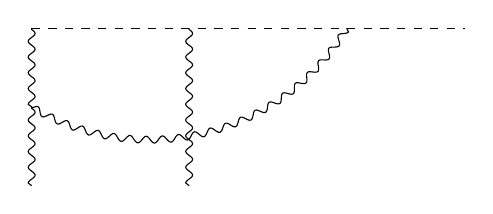
\begin{tikzpicture}
\begin{feynman}
\vertex(field);
\vertex[right=2.0cm of field](wilsontwist1);
\vertex[right=3.5cm of wilsontwist1](infinity);
\vertex[right=2.0cm of wilsontwist1](wilsoncoupling);
\vertex[below=1cm of field](3gluon);
\vertex[below=1cm of 3gluon](outgoingfield);
\vertex[below=2cm of wilsontwist1](outgoingwilsontwist1);
\diagram* {(field) -- [scalar] (infinity)};
\diagram* {(field) -- [boson] (3gluon) -- [boson, quarter right] (wilsoncoupling)};
\diagram* {(3gluon) -- [boson] (outgoingfield)};
\diagram* {(wilsontwist1) -- [boson] (outgoingwilsontwist1)};
\vertex[left=0.5cm of infinity](auxpoint);
\vertex[below=1.5cm of auxpoint](label){\(\thelable\)};
\end{feynman}
\end{tikzpicture}
\vspace{1cm}\hspace{0.5cm}
\def \thelable {B}
\begin{tikzpicture}
\begin{feynman}
\vertex(field);
\vertex[right=2.0cm of field](wilsontwist1);
\vertex[right=3.5cm of wilsontwist1](infinity);
\vertex[right=1.0cm of field](wilsoncoupling);
\vertex[below=1cm of wilsontwist1](3gluon);
\vertex[below=2cm of field](outgoingfield);
\vertex[below=2cm of wilsontwist1](outgoingwilsontwist1);
\diagram* {(field) -- [scalar] (infinity)};
\diagram* {(field) -- [boson] (outgoingfield)};
\diagram* {(wilsontwist1) -- [boson] (3gluon) -- [boson] (outgoingwilsontwist1)};
\diagram* {(wilsoncoupling) -- [boson, quarter right] (3gluon)};
\vertex[left=0.5cm of infinity](auxpoint);
\vertex[below=1.5cm of auxpoint](label){\(\thelable\)};
\end{feynman}
\end{tikzpicture}
\vspace{1cm}
\def \thelable {B'}
\begin{tikzpicture}
\begin{feynman}
\vertex(field);
\vertex[right=2.0cm of field](wilsontwist1);
\vertex[right=3.5cm of wilsontwist1](infinity);
\vertex[right=1.0cm of wilsontwist1](wilsoncoupling);
\vertex[below=1cm of wilsontwist1](3gluon);
\vertex[below=2cm of field](outgoingfield);
\vertex[below=2cm of wilsontwist1](outgoingwilsontwist1);
\diagram* {(field) -- [scalar] (infinity)};
\diagram* {(field) -- [boson] (outgoingfield)};
\diagram* {(wilsontwist1) -- [boson] (3gluon) -- [boson] (outgoingwilsontwist1)};
\diagram* {(wilsoncoupling) -- [boson, quarter left] (3gluon)};
\vertex[left=0.5cm of infinity](auxpoint);
\vertex[below=1.5cm of auxpoint](label){\(\thelable\)};
\end{feynman}
\end{tikzpicture}
\vspace{1cm}\hspace{0.5cm}
\def \thelable {C}
\begin{tikzpicture}
\begin{feynman}
\vertex(field);
\vertex[right=2.0cm of field](wilsontwist1);
\vertex[right=3.5cm of wilsontwist1](infinity);
\vertex[below=1cm of field](3gluon);
\vertex[below=1cm of wilsontwist1](3gluon2);
\vertex[below=2cm of field](outgoingfield);
\vertex[below=2cm of wilsontwist1](outgoingwilsontwist1);
\diagram* {(field) -- [scalar] (infinity)};
\diagram* {(field) -- [boson] (3gluon) -- [boson] (3gluon2) -- [boson] (wilsontwist1)};
\diagram* {(3gluon) -- [boson] (outgoingfield)};
\diagram* {(3gluon2) -- [boson] (outgoingwilsontwist1)};
\vertex[left=0.5cm of infinity](auxpoint);
\vertex[below=1.5cm of auxpoint](label){\(\thelable\)};
\end{feynman}
\end{tikzpicture}
\vspace{1cm}\hspace{0.5cm}
\def \thelable {D}
\begin{tikzpicture}
\begin{feynman}
\vertex(field);
\vertex[right=2.0cm of field](wilsontwist1);
\vertex[right=3.5cm of wilsontwist1](infinity);
\vertex[right=1.0cm of wilsontwist1](wilsoncoupling);
\vertex[right=1.0cm of field](aux4gluon);
\vertex[below=1cm of aux4gluon](4gluon);
\vertex[below=2cm of field](outgoingfield);
\vertex[below=2cm of wilsontwist1](outgoingwilsontwist1);
\diagram* {(field) -- [scalar] (infinity)};
\diagram* {(field) -- [boson] (4gluon) -- [boson] (wilsontwist1)};
\diagram* {(4gluon) -- [boson] (outgoingfield)};
\diagram* {(4gluon) -- [boson] (outgoingwilsontwist1)};
\vertex[left=0.5cm of infinity](auxpoint);
\vertex[below=1.5cm of auxpoint](label){\(\thelable\)};
\end{feynman}
\end{tikzpicture}
\vspace{1cm}
\def \thelable {A1}
\begin{tikzpicture}
\begin{feynman}
\vertex(field);
\vertex[right=2.0cm of field](wilsontwist1);
\vertex[right=3.5cm of wilsontwist1](infinity);
\vertex[right=1.0cm of field](wilsoncoupling);
\vertex[below=2cm of field](outgoingfield);
\vertex[below=2cm of wilsontwist1](outgoingwilsontwist1);
\diagram* {(field) -- [scalar] (infinity)};
\diagram* {(field) -- [boson] (outgoingfield)};
\diagram* {(wilsontwist1) -- [boson] (outgoingwilsontwist1)};
\diagram* {(wilsoncoupling) -- [boson, quarter left] (field)};
\vertex[left=0.5cm of infinity](auxpoint);
\vertex[below=1.5cm of auxpoint](label){\(\thelable\)};
\end{feynman}
\end{tikzpicture}
\vspace{1cm}\hspace{0.5cm}
\def \thelable {A1'}
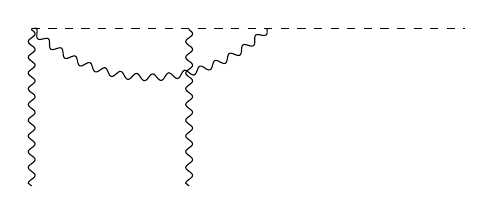
\begin{tikzpicture}
\begin{feynman}
\vertex(field);
\vertex[right=2.0cm of field](wilsontwist1);
\vertex[right=3.5cm of wilsontwist1](infinity);
\vertex[right=1.0cm of wilsontwist1](wilsoncoupling);
\vertex[below=2cm of field](outgoingfield);
\vertex[below=2cm of wilsontwist1](outgoingwilsontwist1);
\diagram* {(field) -- [scalar] (infinity)};
\diagram* {(field) -- [boson] (outgoingfield)};
\diagram* {(wilsontwist1) -- [boson] (outgoingwilsontwist1)};
\diagram* {(wilsoncoupling) -- [boson, quarter left] (field)};
\vertex[left=0.5cm of infinity](auxpoint);
\vertex[below=1.5cm of auxpoint](label){\(\thelable\)};
\end{feynman}
\end{tikzpicture}
\vspace{1cm}\hspace{0.5cm}
\def \thelable {B1}
\begin{tikzpicture}
\begin{feynman}
\vertex(field);
\vertex[right=2.0cm of field](wilsontwist1);
\vertex[right=3.5cm of wilsontwist1](infinity);
\vertex[right=1.0cm of field](wilsoncoupling);
\vertex[below=2cm of field](outgoingfield);
\vertex[below=2cm of wilsontwist1](outgoingwilsontwist1);
\diagram* {(field) -- [scalar] (infinity)};
\diagram* {(field) -- [boson] (outgoingfield)};
\diagram* {(wilsontwist1) -- [boson] (outgoingwilsontwist1)};
\diagram* {(wilsoncoupling) -- [boson, quarter right] (wilsontwist1)};
\vertex[left=0.5cm of infinity](auxpoint);
\vertex[below=1.5cm of auxpoint](label){\(\thelable\)};
\end{feynman}
\end{tikzpicture}
\vspace{1cm}
\def \thelable {B1'}
\begin{tikzpicture}
\begin{feynman}
\vertex(field);
\vertex[right=2.0cm of field](wilsontwist1);
\vertex[right=3.5cm of wilsontwist1](infinity);
\vertex[right=1.0cm of wilsontwist1](wilsoncoupling);
\vertex[below=2cm of field](outgoingfield);
\vertex[below=2cm of wilsontwist1](outgoingwilsontwist1);
\diagram* {(field) -- [scalar] (infinity)};
\diagram* {(field) -- [boson] (outgoingfield)};
\diagram* {(wilsontwist1) -- [boson] (outgoingwilsontwist1)};
\diagram* {(wilsoncoupling) -- [boson, quarter left] (wilsontwist1)};
\vertex[left=0.5cm of infinity](auxpoint);
\vertex[below=1.5cm of auxpoint](label){\(\thelable\)};
\end{feynman}
\end{tikzpicture}
\vspace{1cm}\hspace{0.5cm}
\def \thelable {AB}
\begin{tikzpicture}
\begin{feynman}
\vertex(field);
\vertex[right=2.0cm of field](wilsontwist1);
\vertex[right=3.5cm of wilsontwist1](infinity);
\vertex[below=2cm of field](outgoingfield);
\vertex[below=2cm of wilsontwist1](outgoingwilsontwist1);
\diagram* {(field) -- [scalar] (infinity)};
\diagram* {(field) -- [boson] (outgoingfield)};
\diagram* {(wilsontwist1) -- [boson] (outgoingwilsontwist1)};
\diagram* {(wilsontwist1) -- [boson, quarter left] (field)};
\vertex[left=0.5cm of infinity](auxpoint);
\vertex[below=1.5cm of auxpoint](label){\(\thelable\)};
\end{feynman}
\end{tikzpicture}
\vspace{1cm}\hspace{0.5cm}
\def \thelable {A2}
\begin{tikzpicture}
\begin{feynman}
\vertex(field);
\vertex[right=2.0cm of field](wilsontwist1);
\vertex[right=3.5cm of wilsontwist1](infinity);
\vertex[below=2cm of field](outgoingfield);
\vertex[below=2cm of wilsontwist1](outgoingwilsontwist1);
\vertex[below=1cm of field](3gluon);
\diagram* {(field) -- [scalar] (infinity)};
\diagram* {(field) -- [boson] (3gluon) -- [boson, half right] (field)};
\diagram* {(wilsontwist1) -- [boson] (outgoingwilsontwist1)};
\diagram* {(3gluon) -- [boson] (outgoingfield)};
\vertex[left=0.5cm of infinity](auxpoint);
\vertex[below=1.5cm of auxpoint](label){\(\thelable\)};
\end{feynman}
\end{tikzpicture}
\vspace{1cm}
\def \thelable {B2}
\begin{tikzpicture}
\begin{feynman}
\vertex(field);
\vertex[right=2.0cm of field](wilsontwist1);
\vertex[right=3.5cm of wilsontwist1](infinity);
\vertex[below=2cm of field](outgoingfield);
\vertex[below=2cm of wilsontwist1](outgoingwilsontwist1);
\vertex[below=1cm of wilsontwist1](3gluon);
\diagram* {(field) -- [scalar] (infinity)};
\diagram* {(wilsontwist1) -- [boson] (3gluon) -- [boson, half right] (wilsontwist1)};
\diagram* {(field) -- [boson] (outgoingfield)};
\diagram* {(3gluon) -- [boson] (outgoingwilsontwist1)};
\vertex[left=0.5cm of infinity](auxpoint);
\vertex[below=1.5cm of auxpoint](label){\(\thelable\)};
\end{feynman}
\end{tikzpicture}
\vspace{1cm}
\def \thelable {E1}
\begin{tikzpicture}
\begin{feynman}
\vertex(field);
\vertex[right=2.0cm of field](wilsontwist1);
\vertex[right=3.5cm of wilsontwist1](infinity);
\vertex[below=2cm of field](outgoingfield);
\vertex[below=2cm of wilsontwist1](outgoingwilsontwist1);
\vertex[right=0.5cm of field](wilsoncoupling1);
\vertex[right=1.5cm of field](wilsoncoupling2);
\diagram* {(field) -- [scalar] (infinity)};
\diagram* {(field) -- [boson] (outgoingfield)};
\diagram* {(wilsontwist1) -- [boson] (outgoingwilsontwist1)};
\diagram* {(wilsoncoupling1) -- [boson, half right] (wilsoncoupling2)};
\vertex[left=0.5cm of infinity](auxpoint);
\vertex[below=1.5cm of auxpoint](label){\(\thelable\)};
\end{feynman}
\end{tikzpicture}
\vspace{1cm}
\def \thelable {E2}
\begin{tikzpicture}
\begin{feynman}
\vertex(field);
\vertex[right=2.0cm of field](wilsontwist1);
\vertex[right=3.5cm of wilsontwist1](infinity);
\vertex[below=2cm of field](outgoingfield);
\vertex[below=2cm of wilsontwist1](outgoingwilsontwist1);
\vertex[right=1cm of field](wilsoncoupling1);
\vertex[right=1cm of wilsontwist1](wilsoncoupling2);
\diagram* {(field) -- [scalar] (infinity)};
\diagram* {(field) -- [boson] (outgoingfield)};
\diagram* {(wilsontwist1) -- [boson] (outgoingwilsontwist1)};
\diagram* {(wilsoncoupling1) -- [boson, half right] (wilsoncoupling2)};
\vertex[left=0.5cm of infinity](auxpoint);
\vertex[below=1.5cm of auxpoint](label){\(\thelable\)};
\end{feynman}
\end{tikzpicture}
\vspace{1cm}
\def \thelable {E3}
\begin{tikzpicture}
\begin{feynman}
\vertex(field);
\vertex[right=2.0cm of field](wilsontwist1);
\vertex[right=3.5cm of wilsontwist1](infinity);
\vertex[below=2cm of field](outgoingfield);
\vertex[below=2cm of wilsontwist1](outgoingwilsontwist1);
\vertex[right=0.5cm of wilsontwist1](wilsoncoupling1);
\vertex[right=1.5cm of wilsontwist1](wilsoncoupling2);
\diagram* {(field) -- [scalar] (infinity)};
\diagram* {(field) -- [boson] (outgoingfield)};
\diagram* {(wilsontwist1) -- [boson] (outgoingwilsontwist1)};
\diagram* {(wilsoncoupling1) -- [boson, half right] (wilsoncoupling2)};
\vertex[left=0.5cm of infinity](auxpoint);
\vertex[below=1.5cm of auxpoint](label){\(\thelable\)};
\end{feynman}
\end{tikzpicture}
\\

\ifdefined\mainprogram{}
\else
\end{document}

\fi